\documentclass{beamer} 

\usepackage{filecontents}
\usepackage{graphicx}

% Use classyslides theme and pass options
\usetheme[%
  fonts%
  , header%
  , footer%
  , backgrounds%
  , colors=light%
]{classyslides}
\pgfkeys{/classyslides/backgrounds/.cd, image=primes}
\pgfkeys{/classyslides/backgrounds/.cd, opacity=0.2}
\mode<presentation>

\title{There Is No Largest Prime Number}
\author[Euclid]{Euclid of Alexandria \\ euclid@alexandria.edu}
\date{\today}

% Bibliography
\begin{filecontents}{euclid.bib}
  @book{Labov1972,
    Address = {Philadelphia},
    Author = {William Labov},
    Publisher = {University of Pennsylvania Press},
    Title = {Sociolinguistic Patterns},
    Year = {1972}}

@book{Chomsky1957,
    Address = {The Hague},
    Author = {Noam Chomsky},
    Publisher = {Mouton},
    Title = {Syntactic Structures},
    Year = {1957}}
}

@online{wikipedia-euclid,
  url={https://upload.wikimedia.org/wikipedia/commons/3/30/Euklid-von-Alexandria_1.jpg},
  urldate={2018-10-22}
}

@online{wikipedia:sieve,
  url={https://en.wikipedia.org/wiki/Sieve_of_Eratosthenes},
  urldate={2018-10-29}
}
\end{filecontents}
\addbibresource{./euclid.bib}

%
% Document 
%
\begin{document}

\frame[hide footer, hide header, show background]{
\titlepage
}

%! Table of contents.

\begin{frame}
  \frametitle{Outline}
  \tableofcontents
\end{frame}

\section{Motivation}
\subsection{The Basic Problem That We Studied}

\frame[hide footer, hide header, show background]{
  \sectionpage
}

\begin{frame}[allowframebreaks]
  \frametitle{What Are Prime Numbers?}
  \begin{Definition}{Prime number}
    A \emph{prime number} is a number that has exactly two divisors.
  \end{Definition}
  \framebreak
  \begin{Example}
    \begin{itemize}
      \item 2 is prime (two divisors: 1 and 2).
      \item 3 is prime (two divisors: 1 and 3).
      \item 4 is not prime (\alert{three} divisors: 1, 2, and 4).
    \end{itemize}
  \end{Example}
\end{frame}

\begin{frame}[fragile]
  \frametitle{There Is No Largest Prime Number}%
  \begin{Theorem}{Prime numbers}
    There is no largest prime number.
  \end{Theorem}
\end{frame}

\begin{frame}[fragile]
  \frametitle{There Is No Largest Prime Number}%
  \begin{Proof}
    \begin{enumerate}
      \item<1-> Suppose $p$ were the largest prime number.
      \item<2-> Let $q$ be the product of the first $p$ numbers.
      \item<3-> Then $q + 1$ is not divisible by any of them.
      \item<4-> But $q + 1$ is greater than $1$, thus divisible by some prime number not in the first $p$ numbers.\qedhere
    \end{enumerate}
  \end{Proof}
  \uncover<4->{The proof used \textit{reductio ad absurdum}.}
\end{frame}

\begin{frame}[t]
  \frametitle{What's Still To Do?}
  \begin{itemize}
    \item Answered Questions
    \begin{itemize}
      \item How many primes are there?
    \end{itemize}
    \item Open Questions
    \begin{itemize}
      \item Is every even number the sum of two primes?
    \end{itemize}
  \end{itemize}
\end{frame}

\begin{frame}[fragile, allowframebreaks]
  \frametitle{An Algorithm For Finding Prime Numbers.}
  \begin{Code}{FindPrimeNumbers}
Input: an integer n > 1.

Let A be an array of Boolean values, indexed by integers 2 to n,
initially all set to true.

for i = 2, 3, 4, ..., not exceeding $\sqrt n$:
  if A[i] is true:
    for j = i2, i2+i, i2+2i, i2+3i, ..., not exceeding n:
      A[j] := false.

Output: all i such that A[i] is true.
  \end{Code}
  cf. \cite{wikipedia:sieve}
\end{frame}

\frame{
  \frametitle{It's me, Euclid}
  \begin{figure}
    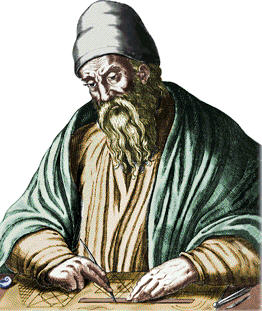
\includegraphics[height=0.6\textheight]{./euclid.jpg}
    \caption{It's me, Euclid \cite{wikipedia-euclid}}
  \end{figure}
}

\nocite{*}
\begin{frame}[allowframebreaks]
  \frametitle{References}
  \printbibliography
\end{frame}
\end{document}